% !TeX spellcheck = en_EN-English
\documentclass[a4paper]{article}
\usepackage[slovak]{babel}
\usepackage[utf8]{inputenc}
\usepackage[T1]{fontenc}
\usepackage{a4wide}
\usepackage{amsmath}
\usepackage{amsfonts}
\usepackage{amssymb}
\usepackage{mathrsfs}
\usepackage[small,bf]{caption}
\usepackage{subcaption}
\usepackage{xcolor}
\usepackage{graphicx}
\usepackage{enumerate}
\usepackage{hyperref}



\pagestyle{empty}
\setlength{\parindent}{0pt}

\newenvironment{modenumerate}
{\enumerate\setupmodenumerate}
{\endenumerate}

\newif\ifmoditem
\newcommand{\setupmodenumerate}{%
	\global\moditemfalse
	\let\origmakelabel\makelabel
	\def\moditem##1{\global\moditemtrue\def\mesymbol{##1}\item}%
	\def\makelabel##1{%
		\origmakelabel{##1\ifmoditem\rlap{\mesymbol}\fi\enspace}%
		\global\moditemfalse}%
}

\renewcommand{\thesubsection}{\alph{subsection})}

\makeatletter
\def\@seccntformat#1{%
	\expandafter\ifx\csname c@#1\endcsname\c@section\else
	\csname the#1\endcsname\quad
	\fi}
\makeatother

\begin{document} 
	
	\pagenumbering{arabic}
	\pagestyle{plain}
	
	\begin{center}
		\sc\large
		MBI Homework 3 for CS students
	\end{center}
	
	Autor: Marián Kravec
	
	\subsection{}
	
	%\centerline{\includegraphics[width=0.7\textwidth]{podorysy}} 
	
	To compute structure with maximal number of base pairs without any not nested cases we will use slightly modified Nussinov algorithm.
	
	\centerline{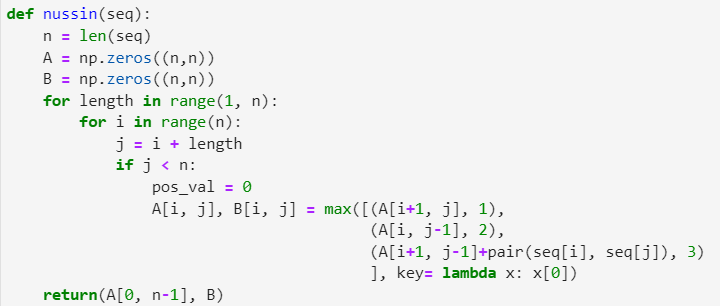
\includegraphics[width=0.7\textwidth]{nussin_1}}
	
	This algorithm is filling out table $A$ (starting from diagonal and getting closer to upper-top corner) where $A[i, j]$ is number maximal number of nested base pair of sub-sequence starting from position $i$ and ending on position $j$ (final solution is in cell $A[0, n]$ where $n$ is length of sequence), it's a bit simple than standard Nussinov algorithm because it does not take into account situation where branching of secondary structure create more base pairs, so situation where we are looking for position $k$ between positions $i$ and  $j$ such that $A[i, k]+A[k+1, j]$ is bigger than any other solution. We omit this rules because breaching creates not nested pairs.
	\\
	\\
	So to compute $A[i, j]$ our algorithm choose maximal value out of three possibilities: $A[i+1, j]$, $A[i, j-1]$ or $A[i+1, j-1]+pair(x_i, x_j)$. 
	\begin{itemize}
		\item{$A[i+1, j]$} - first base of sub-sequence in unpaired and rest is optimally paired 
		\item{$A[i+1, j]$} - last base of sub-sequence in unpaired and rest is optimally paired 
		\item{$A[i+1, j-1]+pair(x_i, x_j)$} - interpretation of this depends on value of $pair(x_i, x_j)$ if $x_i$ and $x_j$ creates pair then this is situation where we take optimal pairing of bases between them plus their own, if they do not create pair then this is situation where we take optimal pairing ob bases between them and first and last base is unpaired
	\end{itemize}
	
	% ADD SOMETHING ABOUT INTERPRETETATION OF STRUCTURE AS LIST OF BASE PAIR
	
	This algorithm compute half of values of matrix with size $n \times n$ and for each position if finds maximum of constant amount of possibilities (only 3), so asymptotic running time of this algorithm is $O(n^2)$.
	
	\subsection{}
	
	Similarly to algorithm from part a), our stochastic context-free grammar needs only one nonterminal which we will call $S$ and to have only three types of rules (three types does not mean three rules), and that is rules to create unpaired bases before nonterminal, rules to create unpaired bases after nonterminal and rules to create pairs (and lastly there will be rule to terminate sequence generation):
	
	\begin{align*}
		S \rightarrow & aS | uS | cS | gS |
		\\
		&Sa | Su | Sc | Sg | 
		\\
		&aSu | uSa | cSg | gSc |
		\\
		&\epsilon 
	\end{align*}
	
\end{document}